%
% $File: report.tex
% $Date: Mon Nov 04 21:48:03 2013 +0800
% $Author: Xinyu Zhou <zxytim@gmail.com>
%

\documentclass{article}
\usepackage{fontspec}
\usepackage{zhspacing,url,amsmath,amssymb,verbatim}
\usepackage{pdfpages}
\zhspacing
\usepackage{listings}
\usepackage[hyperfootnotes=false,colorlinks,linkcolor=blue,anchorcolor=blue,citecolor=blue]{hyperref}
\usepackage[sorting=none]{biblatex}
%\usepackage[dvips]{graphicx}
\usepackage{graphicx}
\usepackage{minted}
\usepackage{subfigure}
\usepackage{indentfirst}
\usepackage{cases}
\usepackage{environ}
\usepackage{array}
\usepackage[top=1in, bottom=1in, left=1.25in, right=1.25in]{geometry}
\usepackage{caption}
%\usepackage{tikz}
%\usepackage{dot2texi}

% $File: mint-defs.tex
% $Date: Thu Sep 26 22:11:33 2013 +0800
% $Author: Xinyu Zhou <zxytim@gmail.com>

\newcommand{\inputmintedConfigured}[3][]{\inputminted[fontsize=\footnotesize,
	label=#3,linenos,frame=lines,framesep=0.8em,tabsize=4,#1]{#2}{#3}}

\newcommand{\txtsrc}[2][]{\inputmintedConfigured[#1]{text}{#2}}
\newcommand{\txtsrcpart}[4][]{\txtsrc[firstline=#3,firstnumber=#3,lastline=#4,#1]{#2}}

\newcommand{\cppsrc}[2][]{\inputmintedConfigured[#1]{cpp}{#2}}
\newcommand{\cppsrcpart}[4][]{\cppsrc[firstline=#3,firstnumber=#3,lastline=#4,#1]{#2}}

\newcommand{\javasrc}[2][]{\inputmintedConfigured[#1]{java}{#2}}
\newcommand{\javasrcpart}[4][]{\javasrc[firstline=#3,firstnumber=#3,lastline=#4,#1]{#2}}

\newcommand{\matlabsrc}[2][]{\inputmintedConfigured[#1]{matlab}{#2}}
\newcommand{\matlabsrcpart}[4][]{\matlabsrc[firstline=#3,firstnumber=#3,lastline=#4,#1]{#2}}

%\usepackage[T1]{fontenc}
\usepackage{lmodern}
\usepackage{amssymb,amsmath}
\usepackage{ifxetex,ifluatex}
\usepackage{fixltx2e} % provides \textsubscript
% use upquote if available, for straight quotes in verbatim environments
\IfFileExists{upquote.sty}{\usepackage{upquote}}{}
\ifnum 0\ifxetex 1\fi\ifluatex 1\fi=0 % if pdftex
  \usepackage[utf8]{inputenc}
\else % if luatex or xelatex
  \usepackage{fontspec}
  % commented by Xinyu Zhou
  \ifxetex
    \usepackage{xltxtra,xunicode}
  \fi
  \defaultfontfeatures{Mapping=tex-text,Scale=MatchLowercase}
  \newcommand{\euro}{€}
\fi
% use microtype if available
\IfFileExists{microtype.sty}{\usepackage{microtype}}{}
\usepackage{color}
\usepackage{fancyvrb}
\newcommand{\VerbBar}{|}
\DefineShortVerb[commandchars=\\\{\}]{\|}
\DefineVerbatimEnvironment{Highlighting}{Verbatim}{commandchars=\\\{\}}
% Add ',fontsize=\small' for more characters per line
\newenvironment{Shaded}{}{}
\newcommand{\KeywordTok}[1]{\textcolor[rgb]{0.00,0.44,0.13}{\textbf{{#1}}}}
\newcommand{\DataTypeTok}[1]{\textcolor[rgb]{0.56,0.13,0.00}{{#1}}}
\newcommand{\DecValTok}[1]{\textcolor[rgb]{0.25,0.63,0.44}{{#1}}}
\newcommand{\BaseNTok}[1]{\textcolor[rgb]{0.25,0.63,0.44}{{#1}}}
\newcommand{\FloatTok}[1]{\textcolor[rgb]{0.25,0.63,0.44}{{#1}}}
\newcommand{\CharTok}[1]{\textcolor[rgb]{0.25,0.44,0.63}{{#1}}}
\newcommand{\StringTok}[1]{\textcolor[rgb]{0.25,0.44,0.63}{{#1}}}
\newcommand{\CommentTok}[1]{\textcolor[rgb]{0.38,0.63,0.69}{\textit{{#1}}}}
\newcommand{\OtherTok}[1]{\textcolor[rgb]{0.00,0.44,0.13}{{#1}}}
\newcommand{\AlertTok}[1]{\textcolor[rgb]{1.00,0.00,0.00}{\textbf{{#1}}}}
\newcommand{\FunctionTok}[1]{\textcolor[rgb]{0.02,0.16,0.49}{{#1}}}
\newcommand{\RegionMarkerTok}[1]{{#1}}
\newcommand{\ErrorTok}[1]{\textcolor[rgb]{1.00,0.00,0.00}{\textbf{{#1}}}}
\newcommand{\NormalTok}[1]{{#1}}
% \ifxetex
%   \usepackage[setpagesize=false, % page size defined by xetex
%               unicode=false, % unicode breaks when used with xetex
%               xetex]{hyperref}
% \else
%   \usepackage[unicode=true]{hyperref}
% \fi
\hypersetup{breaklinks=true,
            bookmarks=true,
            pdfauthor={},
            pdftitle={},
            colorlinks=true,
            urlcolor=blue,
            %linkcolor=magenta,
            pdfborder={0 0 0}}
%\urlstyle{same}  % don't use monospace font for urls
\setlength{\parindent}{0pt}
\setlength{\parskip}{6pt plus 2pt minus 1pt}
\setlength{\emergencystretch}{3em}  % prevent overfull lines
%\setcounter{secnumdepth}{0}



\newcommand{\figref}[1]{\hyperref[fig:#1]{Figure\ref*{fig:#1}}}
\newcommand{\tableref}[1]{\hyperref[table:#1]{Table\ref*{table:#1}}}
\newcommand{\centerize}[1]{\begin{center} #1 \end{center}}

\newcommand{\cmd}[1]{{\it #1}}
\newcommand{\ccmd}[1]{\centerize{\cmd{#1}}}

\title{Digital Signal Processing: Speaker Recognition}
\author{Xinyu Zhou, Yuxin Wu, and Tiezheng Li\\ Tsinghua University}
\date{\today}

\addbibresource{refs.bib}
\begin{document}
\maketitle
\section{Introduction}
A \textbf{Speaker Recognition} tasks can be classified with respect to diffenrent criterion:
Text-dependent or Text-independent, Verification (decide whether the person is he claimed
to be) or Identification (decide who the person is by its voice).\cite{SRwiki}

Speaker recognition is an important part of Human-Computer Interaction (HCI).
As the trend of employing wearable computer reveals, Voice User Interface (VUI)
has been a vital part of such computer. As these devices are particularly small,
the are more likely to lose and be stolen. In these scenario, speaker recognition
is not only a good HCI, but also a combination of seamless interaction with computer
and security guard when the device is lost.

Further more, these techniques can be used in environment which demands high security.
It can be combined with other biological metrics to form a multi-modal authentication
system.

In this task, our goal is to build a proof-of-concept text-dependent speaker recognition system with GUI support.
Hopefully, we would like to extend its ability to a text-independent speaker recognition system.

\section{Approach}

The task of speaker recognition can be considered as a task of classification. Thus a number of machine learning techniques
can be applied to this task. In general, this task should cover the following three topics:
\begin{enumerate}
  \item Feature Extraction: process the voice signal and describe it with features.

  \item Acoustic Model: provide the functionality of registration as well as identification or verification.

  \item Testing: test the precision and accuracy of our system
\end{enumerate}

\subsection{Feature Extraction}
The task of speaker recognition is highly correlated to the task of speech recognition.
In the field of speech recognition, Complex Cepstrum \cite{cepstrum} is
considered to be a concise description to the original acoustic signal.
In particular, Mel-frequency Cepstral Coefficients (MFCC), is a state-of-the-art standard feature
widely used in Automatic Speech Recognition (ASR) system.
The general procedure for calculating MFCC is as follows:
\begin{figure}[H]
  \centering
  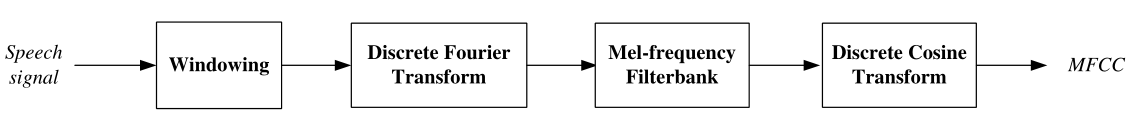
\includegraphics[width=\textwidth]{res/MFCC.png}
\end{figure}

As for speaker recognition, several different features are suggested and compared
by researchers \cite{evaluation}. Cepstrum still proves to be a robust and effective
feature in this task. Therefore, a bunch of cepstral features, including MFCC,
LPCC (Linear Prediction Cepstrum Coefficients), are commonly used
in speaker recognition system.\cite{feature}

We plan to implement common cepstral features used by researchers, and use a
combination of some of them, according to the further observation and test on how
much they contribute to the task.

\subsection{Model}
According to works in years, Gaussian Mixture Model (GMM)
has been a common approach to acoustic modeling.\cite{GMM}
GMM can be used to acquire an acoustic model $P(\mathbf{O} | \mathbf{W}) $,
which gives the probability of a given observation
$\mathbf{O}$ under certain word $\mathbf{W}$. By using GMM, this
conditional probability can be well estimated by modeling the distribution as
a sum of several normal distribution.

In addition to that, Hidden Markov Model (HMM) is a main-stream approach in ASR system,
since it can describe sequential relation of observations.\cite{SLP}
We have noticed a few research-oriented open-source speech recognition
tool building on HMM, such as HTK\cite{htk}.
The techniques and result of such tools might be quite useful in buiding a
speaker recognition system.

Recently, some common machine learning model are also applied to the task of speaker
recognition. \cite{svm} suggested a method of using SVM in speaker recognition.
Deep neural networks are also used in speech processing recently.\cite{deep}

HMM and GMM are our first choices, as they are already widely used and proven to be
efficient and effective.  We might also try to migrate our extracted feature to
some other available models.

\subsection{Testing}
There are a number of well-known data sets for testing in speaker recognition systems,
such as KING speaker verification\cite{king}. \cite{database} gives description on
several common databases. But most of these databases are not free of charge.
We intend to try to search for an freely available database,
otherwise we have to build some simple test cases by our own.

\printbibliography

\end{document}

